\documentclass[pdf]{beamer}
\mode<presentation>{\usetheme{Malmoe}\usecolortheme{dolphin}}
\title{Improving an Exact Solution to the \newline ($l$,$d$) Planted Motif Problem}
\author{Maria Clara Isabel Sia}

\AtBeginSection[]{
	\begin{frame}{}\tableofcontents[currentsection]\end{frame}
}

\begin{document}

\begin{frame}
\titlepage
\end{frame}

\section{Introduction}
	\begin{frame}{Introduction}
		\begin{itemize}
			\item<2-> motifs: repeated sub-sequences in DNA that have some biological significance\newline
			\item<3-> DNA motif finding: search for motifs over a set of DNA sequences, allowing for mismatches due to mutation\newline
			\item<4-> known as a difficult problem in computational biology and CS (proven NP-complete)\newline
		\end{itemize}
		\end{frame}

	\subsection{The ($l$,$d$) planted motif problem}
		\begin{frame}{The ($l$,$d$) planted motif problem}
			\centering{
			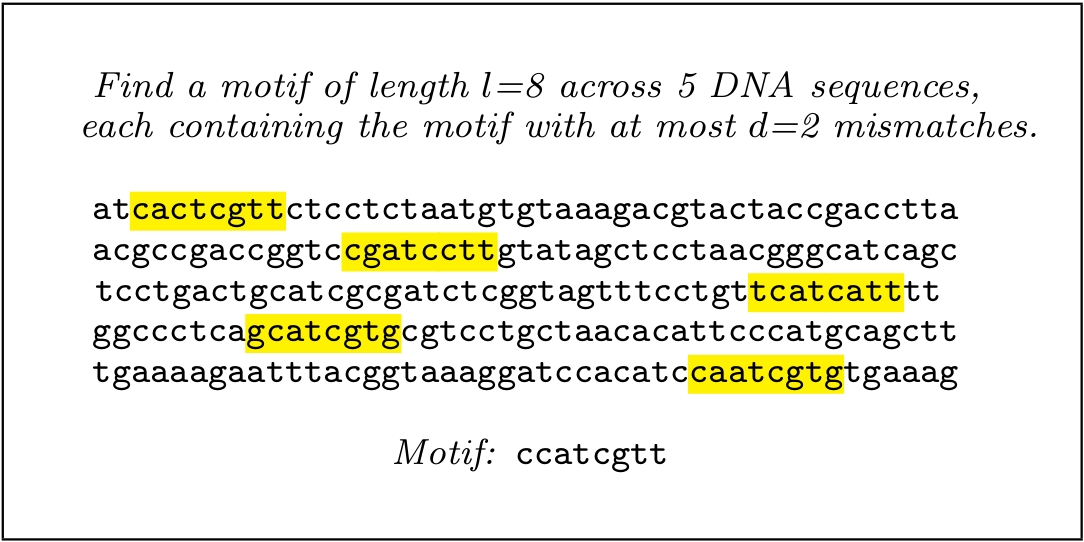
\includegraphics[width=7.5cm]{img/example}
			}\newline

			\uncover<2>{
				Given a set $\mathcal{S} = \{S_{1},...S_{n}\}$ of $n$ DNA sequences of length $L$,
				\newline \hspace*{12pt} find $M$, the set of sub-sequences (motifs) of length $l < L$
				\newline \hspace*{12pt} which occur with at most $d$ mismatches in each sequence in $\mathcal{S}$. %in $S$.
			}

			\end{frame}

	\subsection{Definitions of key concepts}
		\begin{frame}{Definitions of key concepts}
			\begin{itemize}[<1-6>]
			\item $l$-mer
			\only<2>{
				\newline- sequence of length $l$
				\newline
\includegraphics[width=10.0cm]{img/concepts_lmer}
			}
			\item Hamming distance $dH(x_1, x_2)$
			\only<3>{
				\newline- number of mismatches between $l$-mers $x_1$ and $x_2$
				\newline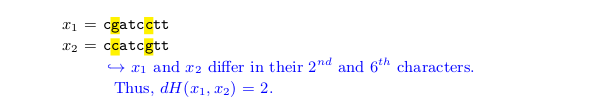
\includegraphics[width=10.0cm]{img/concepts_dH}		
			}
			\item $d$-neighborhood $N(x,d)$ of $l$-mer $x$
			\only<4>{
				\newline- set of all $l$-mers having at most $d$ mismatches with $x$
				\newline\newline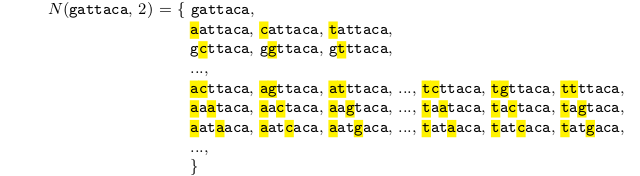
\includegraphics[width=10.0cm]{img/concepts_N(x,d)2}	
			}
			\item $d$-neighborhood $\mathcal{N}(S,d)$ of sequence $S$
			\only<5>{
				\newline- union of $d$-neighborhoods of all $l$-mers in $S$
				\newline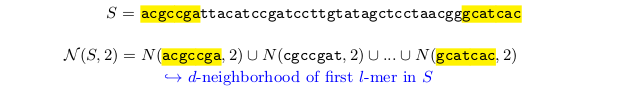
\includegraphics[width=10.0cm]{img/concepts_N(S,d)2}		
			}
			\end{itemize}
			\end{frame}

\section{EMS-GT}
	\subsection{The EMS-GT algorithm}
		\begin{frame}{The EMS-GT algorithm}
			The EMS-GT algorithm proceeds in two main steps:\newline
			\begin{enumerate}
			\item<2-> \emph{Generate candidates}\newline
			\uncover<3->{Take the intersection of the $d$-neighborhoods of the first $n'$ sequences $S_1,S_2,...,S_{n'}$. Every $l$-mer in the resulting set $C$ is a candidate motif.\newline}
			\item<4-> \emph{Test candidates}\newline
			\uncover<5->{For every candidate $c$ in $C$, check whether a $d$-neighbor of $c$ appears in each of the remaining sequences $S_{n'+1},S_{n'+2},...S_n$. If this is the case, accept $c$ as a motif.\newline}
			\end{enumerate}
			\end{frame}

	\subsection{Efficiency strategies}
		\begin{frame}{EMS-GT efficiency strategies}
			\begin{itemize}
			\item $l$-mer enumeration
			\only<2>{\newline}
			\item Bit-based set representation
			\only<3>{\newline}
			\item Recursive neighborhood generation
			\only<4>{\newline}
			\end{itemize}
			\end{frame}

\section{Methodology}
	\subsection{Research objectives}
	\begin{frame}{Methodology}
		The main objectives of this research are:\newline
		\begin{enumerate}
		\item<2-> To develop a speedup technique for EMS-GT that takes advantage of distance-related patterns in the search space;\newline
		\item<3-> To evaluate the speedup technique with regard to improvement in runtime; and\newline
		\item<4> To evaluate the improved version of EMS-GT against state-of-the-art motif search algorithms.
		\end{enumerate}
		\end{frame}
	\subsection{Development and evaluation}
	\begin{frame}{Methodology}
		\begin{itemize}
		\item<1-> \emph{Developing an EMS-GT speedup technique}\newline
		\uncover<2->{In EMS-GT, $l$-mer neighborhoods are represented with repeating patterns of bits. We exploit these patterns in a speedup technique that sets bits quickly and in blocks.\newline}

		\item<3-> \emph{Evaluating performance}\newline
		\uncover<4->{Performance is benchmarked on ``challenging'' ($l$,$d$) instances: (9,2), (11,3), (13,4), (15,5) and (17,6).\newline}

		\begin{itemize}
			\item<5-> \emph{Synthetic datasets}\newline
			\uncover<6->{- sets of 20 randomly-generated DNA sequences of length 600, with the same ($l$,$d$) motif planted once in each sequence.}
		\end{itemize}

		\end{itemize}
		\end{frame}

\section{Results}
	\subsection{Pattern-based speedup technique}
	\begin{frame}{Pattern-based speedup technique}

		\end{frame}

	\subsection{Performance}
	\begin{frame}{Performance improvement with speedup}

		\end{frame}

	\begin{frame}{Performance vs PMS8, qPMS9}

		\end{frame}

\section{Conclusion}

\begin{frame}
	\centering
	Thank you!
\end{frame}
\end{document}